\def\pgfsysdriver{pgfsys-dvisvgm.def}
% flashcards-title: Observed association compared with intervention evidence
% flashcards-desc: Panel A links observed shade and height with a two-headed line. Panel B uses a one-way assigned-shade arrow leading to later height comparison, with matched conditions noted.
\documentclass[tikz,border=6pt]{standalone}
\usetikzlibrary{arrows.meta,calc,fit,positioning,shapes.geometric}

\definecolor{fcink}{HTML}{17212B}
\definecolor{fcblue}{HTML}{1D5D8C}
\definecolor{fcgreen}{HTML}{2D6A4F}
\definecolor{fcorange}{HTML}{A44A1F}
\definecolor{fcpale}{HTML}{F4F7F9}
\definecolor{fcsoil}{HTML}{8B5E3C}

\tikzset{
  fc text/.style={font=\sffamily, text=fcink},
  fc panel/.style={draw=fcink, line width=0.9pt, rounded corners=5pt, fill=fcpale},
  fc node/.style={draw=fcink, line width=0.9pt, rounded corners=4pt, fill=white,
    minimum width=24mm, minimum height=10mm, align=center, font=\sffamily},
  fc arrow/.style={-{Stealth[length=3.2mm,width=2.4mm]}, line width=1.2pt,
    draw=fcblue, line cap=butt},
  fc boundary/.style={draw=fcorange, line width=1.4pt, dash pattern=on 5pt off 3pt,
    rounded corners=7pt},
  fc label/.style={font=\sffamily\bfseries, text=fcink},
  fc note/.style={font=\sffamily\small, text=fcink, align=center}
}

\begin{document}
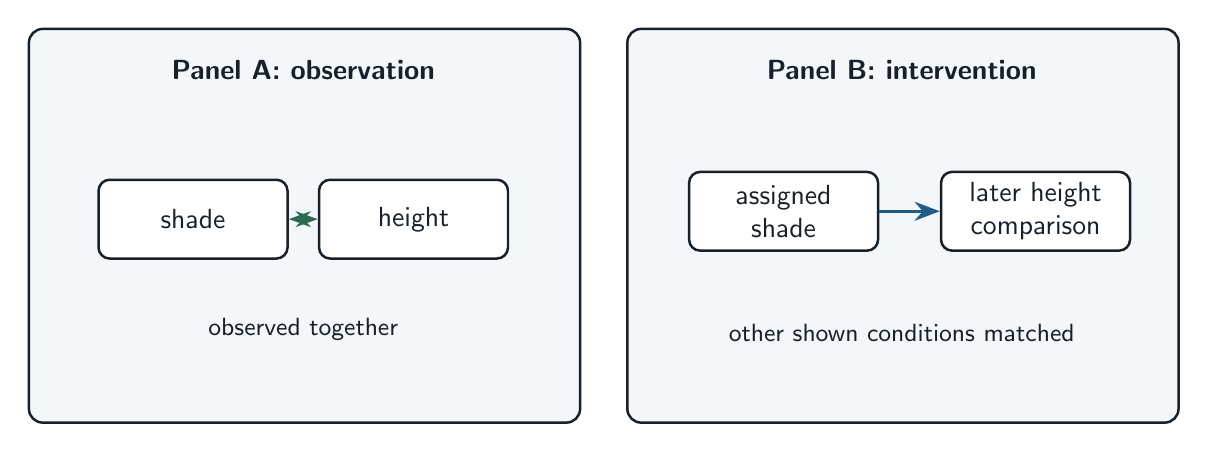
\begin{tikzpicture}[fc text, x=1cm, y=1cm]
  \node[fc panel, minimum width=70mm, minimum height=50mm, anchor=south west] at (0,0) {};
  \node[fc panel, minimum width=70mm, minimum height=50mm, anchor=south west] at (7.6,0) {};
  \node[fc label] at (3.5,4.5) {Panel A: observation};
  \node[fc node] (shadeA) at (2.1,2.6) {shade};
  \node[fc node] (heightA) at (4.9,2.6) {height};
  \draw[{Stealth[length=2.8mm,width=2mm]}-{Stealth[length=2.8mm,width=2mm]}, draw=fcgreen, line width=1.2pt] (shadeA)--(heightA);
  \node[fc note] at (3.5,1.2) {observed together};
  \node[fc label] at (11.1,4.5) {Panel B: intervention};
  \node[fc node] (shadeB) at (9.6,2.7) {assigned\\shade};
  \node[fc node] (heightB) at (12.8,2.7) {later height\\comparison};
  \draw[fc arrow] (shadeB)--(heightB);
  \node[fc note] at (11.1,1.15) {other shown conditions matched};
\end{tikzpicture}
\end{document}
